\section{Process} \label{sec:process}


Throughout the Rubin pre-operations and operations phases, annually in May each team will look back at what was planned, what was achieved, do a full review of its activities, and propose a high level plan for the following (US fiscal) year.
This is standard practice in other high energy physics experiments as well, the scrub allows the facility to continuously evolve its operating plan, taking critical input from the people that understand best what is really needed, in Rubin’s case that is the Team Leaders.
Following the National Science Foundation and Department of Energy joint annual review of Rubin Operations the Rubin Operations Directors office together with department heads sets the major milestones for the next US fiscal year (FY) starting 1st October. This includes looking at the status of major milestones for the current year and ascertaining whether any of those need to carry over into the next FY.
With the major milestones set, the Director’s office kicks off the month long annual scrub process, see \autoref{fig:timeline} in which the department heads start down stream planning with their teams. This is the “homework” phase of the scrub where teams are looking at:

\begin{itemize}
\item status of minor milestones for the current FY
\item setting minor milestones that would contribute to accomplishing the new major milestones for the next FY
\item based on activities needed to achieve the minor milestones and risk mitigation plans the teams review planned resources both labor and non-labor
\item if there is a mismatch between resources needed and the resources available the team will propose changes during this scrub period through the tool (described in the next section).

\end{itemize}


\begin{figure}
\begin{centering}
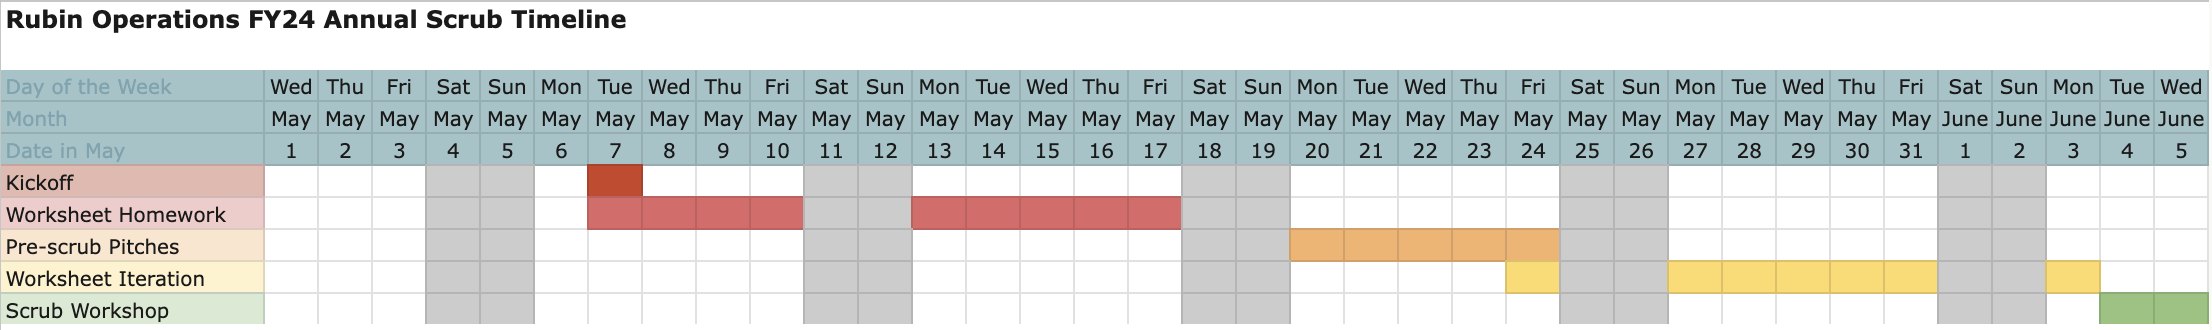
\includegraphics[width=0.9\textwidth]{Figure1Scrubtimeline}
	\caption{Scrub timeline
\label{fig:timeline}}
\end{centering}
\end{figure}
